\documentclass[11pt,a4paper]{article}

% ---------------------------------------------------------------------------
% Certified one-bit chemical computation: finite-fuel correction, productive
% readout, and inheritance.
%
% Author metadata: set the macros below before submission.  They are
% deliberately left blank in this version.  \CompanionAuthor is the author
% printed for the companion manuscripts in refs.bib; \RepositoryNote is where
% the public repository location goes.
% ---------------------------------------------------------------------------
\newcommand{\PaperAuthor}{}
\newcommand{\PaperAffiliation}{}
\newcommand{\PaperDate}{17 September 2026}
\newcommand{\CompanionAuthor}{Anonymous}
\newcommand{\RepositoryNote}{The repository location and a permanent archive of the
sources will be supplied with the author information.}

\usepackage[T1]{fontenc}
\usepackage[utf8]{inputenc}
\usepackage{lmodern}
\usepackage{microtype}
\usepackage[a4paper,margin=1.05in]{geometry}
\usepackage{amsmath,amssymb,amsthm,mathtools}
\usepackage{booktabs}
\usepackage{array}
\usepackage{enumitem}
\usepackage{xcolor}
\usepackage{graphicx}
\usepackage{caption}
\usepackage{tikz}
\usetikzlibrary{arrows.meta,positioning,calc}
\usepackage[obeyspaces,spaces]{url}
\usepackage[numbers,sort&compress]{natbib}
\usepackage[colorlinks=true,linkcolor=blue!55!black,citecolor=blue!55!black,
            urlcolor=blue!55!black]{hyperref}
\hypersetup{pdftitle={Certified one-bit chemical computation: finite-fuel correction,
  productive readout, and inheritance},
  pdfkeywords={chemical computation, stochastic reaction networks, approximate majority,
  finite fuel, compositional inheritance, compartment selection, uniformization, Lean}}

\DeclareUrlCommand\lean{\urlstyle{tt}}
\newcolumntype{R}{>{\raggedright\arraybackslash}p{.303\linewidth}}
\newcolumntype{L}{>{\raggedright\arraybackslash}p{.40\linewidth}}
\newcolumntype{M}{>{\raggedright\arraybackslash}p{.53\linewidth}}
\setlist{itemsep=2pt,topsep=3pt}
\setlength{\emergencystretch}{1.5em}
\captionsetup{font=small,labelfont=bf}
\graphicspath{{figures/}}
\renewcommand{\topfraction}{0.92}
\renewcommand{\bottomfraction}{0.82}
\renewcommand{\textfraction}{0.07}
\renewcommand{\floatpagefraction}{0.80}

\theoremstyle{plain}
\newtheorem{theorem}{Theorem}[section]
\newtheorem{proposition}[theorem]{Proposition}
\newtheorem{lemma}[theorem]{Lemma}
\newtheorem{corollary}[theorem]{Corollary}
\theoremstyle{definition}
\newtheorem{definition}[theorem]{Definition}
\theoremstyle{remark}
\newtheorem{remark}[theorem]{Remark}

\newcommand{\N}{\mathbb N}
\newcommand{\Prob}{\mathbb P}
\newcommand{\E}{\mathbb E}
\newcommand{\B}{\mathcal B}
\newcommand{\ind}{\mathbf 1}
\newcommand{\eps}{\varepsilon}
\newcommand{\ff}[2]{(#1)_{#2}}
\newcommand{\Bin}{\mathrm{Bin}}

\title{Certified one-bit chemical computation:\\[4pt]
\large finite-fuel correction, productive readout, and inheritance}
\author{\PaperAuthor\\[2pt] {\small\itshape \PaperAffiliation}}
\date{\PaperDate}

\begin{document}
\maketitle

\begin{abstract}
A chemical module computes reliably only if the state that encodes its input survives
the act of using it: making the output consumes the same finite material that maintains
the state, and dividing the compartment splits that state at random. We construct a
seven-species reversible count reaction network, with one fuel species, whose
compartment realises a complete one-bit contract. Two preparations with identical
molecular support encode the two input values; the network repairs a bounded number of
wrong-label molecules, delivers at least four molecules of the corresponding product by
a fixed deadline, and returns \emph{both} complementary daughters to the region that
encodes the same value. A single probability bound covers all of these events on one
trajectory. For an $81$-unit preparation we prove a uniform joint guarantee of at least
$0.9997$ over a parameter box that simultaneously spans a hundredfold range in the
correction rate constant, admits product recovery as low as $90\%$, and admits division
bias anywhere in $[0.48,0.52]$;
under ideal operations the same construction gives $0.9998$. The proof combines a
fixed-time reaction-clock comparison with a downward-rounded integer certificate on a
$3\,240$-state core, so that no floating-point matrix exponential enters the argument.
Correction consumes fuel, and its embedded jump chain is exactly solvable: it is the
Mabinogion urn, whose wrong-consensus probability $2^{-(r-3)}$ from two minority
molecules among $r$ residents is independent of how fast the correcting reaction is.
Weighting the exact absorption law by the fuel actually spent yields a $144$-unit,
two-minority construction with joint probability at least $0.9916$, within
$5.5\cdot10^{-4}$ of the ceiling that the consensus law imposes on its worst admitted
state. The same law makes heritable variation quantitative: a specified mixed
preparation produces a productive \emph{opposite}-program daughter pair with probability
above $0.0074$, whereas a pure newborn does so with probability at most $8.1\cdot10^{-6}$,
because on a pure face the only channel that can create a minority molecule is
first-order leakage. No single label-dependent switching rate can therefore describe
both classes of newborn. An external product-dependent retention rule converts the
output distinction into an explicit finite-population selection bound. The probability
theorems are conventional arguments supported by exact finite computation; selected
source, partition, rate and arithmetic lemmas are checked in Lean~4. High-order
reactions, severe kinetic separation and idealised inventory operations remain
assumptions: this is a certified mathematical model of one-bit chemical information
processing, not a calibrated biochemical implementation.
\end{abstract}

\section{Introduction}\label{sec:intro}

\subsection{The contract}

Chemical reaction networks compute. Stochastic reaction networks with a finite number of
molecules are a well-studied model of computation~\citep{soloveichik2008,chen2014,%
cummings2016}, abstract networks can be compiled into DNA~\citep{soloveichik2010,%
qian2011,chen2013}, and specific motifs implement specific primitives: approximate
majority is computed by a population protocol~\citep{angluin2008}, by a tri-molecular
reaction network~\citep{condon2020}, and by the biological cell-cycle
switch~\citep{cardelli2012}.

Almost all of this work certifies a \emph{transient output}: the network is started in a
state encoding the input, and one asks for the distribution of a designated species at a
later time. A physical module that is used repeatedly must satisfy something stronger.
Producing the output consumes material. The compartment holding the state divides, and
the state is split by a random partition that no controller supervises~\citep{huh2011pnas,%
huh2011ng}. If we want to run the module again, the state that remains after paying for
the output and after being cut in half must still be an admissible input state --- for
\emph{both} halves, not for a favourable one.

We therefore fix the following contract, and prove a single probability bound for all of
its clauses \emph{on one trajectory and one partition}. Let the logical input be
$b\in\{X,Y\}$.

\begin{enumerate}[label=(C\arabic*),leftmargin=2.6em]
\item \textbf{Encoding.} $b$ is encoded by the composition of the compartment: an
  admissible encoding is any state of an explicitly specified finite region
  $\B_b^{L,k}$. The two regions have identical molecular support, so the encoder cannot
  be said to hand the network a distinguishing species.
\item \textbf{Correction.} A preparation may contain up to $k$ molecules of the wrong
  label. The network must remove them, using its own fuel, before they corrupt the
  output.
\item \textbf{Productive readout.} At a fixed deadline $T$ the compartment must contain,
  and surrender to an imperfect collection step, at least four molecules of the product
  $P_b$ and at most one molecule of $P_{\bar b}$.
\item \textbf{Inheritance.} After the product is removed and every remaining molecule is
  assigned at random to one of two daughters, \emph{both} daughters, refilled by a
  label-blind procedure, must lie in $\B_b^{L,k}$ again.
\item \textbf{Uniformity.} The guarantee must hold uniformly over all admissible
  encodings of $b$, over an interval of rate constants, and over an interval of
  operation parameters --- not at a single tuned point.
\end{enumerate}

The interesting word is \emph{and}. In our network the reaction that copies a resident
molecule and the reaction that makes the product have the \emph{same} propensity $sf$ and
draw on the \emph{same} finite food pool, so (C3) and (C4) compete for one resource; and
the correction reaction of (C2) burns a fuel molecule that is not replenished during the
batch. The theorem is a statement about a resource conflict, not about a memory model
with an independent reward counter attached.

\subsection{Results}

The source (Table~\ref{tab:source}) has seven species $X,Y,F,P_X,P_Y,H,W$ and seven
reversible pairs, all with positive rate constants in both directions. Its correction
pair, read forward and with the fuel bookkeeping deleted, is $X+X+Y\to 3X$ together with
its label swap: exactly the tri-molecular approximate-majority network of
\citet{condon2020}. What we add is that each correction event consumes one molecule of
fuel $H$ and releases one molecule of waste $W$, that the reverse reaction is present,
and that the correction runs concurrently with the food-consuming reactions that make
the output. The results are the following.

\begin{itemize}[leftmargin=1.2em]
\item \textbf{A joint certificate (Theorem~\ref{thm:main}).} For a compartment holding
  $81$ modelled material units, contract (C1)--(C5) holds with probability at least
  $9997/10000$ in a regime (WO) whose kinetic box spans a hundredfold range in $\gamma$
  and which simultaneously tolerates product recovery
  $\eta\in[0.9,1]$ and division bias $\theta\in[0.48,0.52]$. Restricting either the
  kinetics or the operations gives $4999/5000$.
\item \textbf{A logical reading (Corollaries~\ref{cor:decoder} and \ref{cor:fano}).}
  Fixed decoders of the two daughters and of the collected product all return the input
  bit, with total-variation distance at most $2\cdot 10^{-4}$ (respectively
  $3\cdot10^{-4}$) between the decoded triple and the constant triple $(b,b,b)$; each
  decoded output carries at least $0.9972$ (respectively $0.9960$) bits about a uniformly
  random input bit.
\item \textbf{An exact integer certificate (Proposition~\ref{prop:certificate}).} The
  terminal payoff of a $3\,240$-state pure core is bounded below by a downward-rounded
  integer uniformization recurrence with certified $64$-bit accumulator bounds. No
  floating-point matrix exponential, and no statistical confidence interval, enters any
  claim.
\item \textbf{The fuel law (Theorem~\ref{thm:walk}, Corollary~\ref{cor:inventory}).} The
  embedded correction chain has jump probabilities $(r-j-1)/(r-2)$ and $(j-1)/(r-2)$,
  independent of the rate constant, of the fuel level and of time. Its unlimited-fuel
  absorption probability is the Mabinogion urn law of \citet{flajolet2008}; from two
  minority molecules the wrong-consensus probability is exactly $2^{-(r-3)}$. Hence a
  correction-only route to error $\delta$ needs $r\ge 3+\lceil\log_2(1/\delta)\rceil$
  residents --- no amount of catalytic speed substitutes for inventory.
\item \textbf{Spent fuel as a state variable (Lemma~\ref{lem:spent},
  Theorem~\ref{thm:F}).} Charging each successful trajectory the fuel it actually spent,
  rather than the fuel it was given, improves the two-minority guarantee from
  $0.99010\ldots$ to $0.99164\ldots$ at $144$ units, and the improved bound is within
  $5.5\cdot 10^{-4}$ of the ceiling $127/128$ that Theorem~\ref{thm:walk} imposes on its
  worst admitted state (Remark~\ref{rem:sharp}).
\item \textbf{Variation is not a label-only rate (Theorem~\ref{thm:pure},
  Corollary~\ref{cor:nokernel}).} A specified mixed preparation yields a productive
  \emph{opposite}-program daughter pair with probability $>0.0074$. A pure newborn yields
  one with probability at most $8.1\cdot 10^{-6}$, because on a pure face with no waste
  the majority channels are both disabled and the only minority-creating channel is
  first-order leakage. The two classes differ by a factor above $935$, so no two-state
  mutation matrix indexed by the label alone is consistent with the source.
\item \textbf{Selection (Theorem~\ref{thm:selection}).} An external rule that reads only
  the collected product, never a label, moves the compartment-count odds of a $20$-member
  population from $1:1$ to at least $5:4$ in one round with probability at least
  $16297339/16384000$, with no independence assumption on the chemical failures.
\end{itemize}

\subsection{What is not claimed}\label{sec:notclaimed}

We state the boundary once, and keep to it.

\emph{Not universal computation.} The module stores and transmits one bit and emits one
of two products. ``Program'' means a choice between two product recipes. We do not
compose modules, and the fan-out described here is the copying of one bit into two
compartments, not the production of two independent bits usable by arbitrary downstream
circuits.

\emph{Not a priority claim.} Chemical majority computation~\citep{angluin2008,%
cardelli2012,condon2020}, programmable chemical kinetics~\citep{soloveichik2010,qian2011,%
chen2013}, experimentally programmable autocatalysis~\citep{kriukov2024}, compositional
heredity~\citep{segre2000,matsubara2026} and compartment-level competition and
selection~\citep{matsumura2016,lu2024} all have substantial predecessors. Our
contribution is the joint finite-inventory certificate and the exactly solvable
finite-fuel correction law, not the individual ingredients. We are also not the first to
verify reaction-network statements in a proof assistant~\citep{lathrop2024,ripple2026} or
by probabilistic model checking~\citep{lakin2012,kwiatkowska2011}; our formal component is
modular and its exact boundary is given in Appendix~\ref{app:evidence}.

\emph{Not a physical implementation.} The correction reaction is fourth order in both
directions, and the required kinetic separation is extreme (Section~\ref{sec:physical}).
A candidate elementary mechanism that we examined fails for reasons we quantify in
Section~\ref{sec:elementary} rather than dismiss. Whether \emph{some} elementary
mechanism satisfies the same contract is open, and by \citet{phan2026} the realizability
question is itself hard. The species are abstract; no molecular identities are assigned.

\emph{Not evolution.} We prove one-cycle heritable variation from a specified mixed
preparation and a one-round external selection bound. We do not prove a useful recurrent
mutation rate from the actual descendants of pure newborns; Theorem~\ref{thm:pure} shows
why that is a genuinely different question, and bounds it from the wrong side.

\emph{Not an end-to-end formal proof.} The probability theorems are conventional
arguments supported by exact rational and integer computation. Lean~4 checks the reaction
table and its invariants, the repair clock, the partition identity, the uniformization
and block-iteration lemmas, the prefix maximum, the exponential estimates, the embedded
jump probabilities, the finite-fuel recurrence and the selection tails. It does not
replay the $3\,240$-state recurrence, and an arithmetic theorem about a reported
numerator is not a theorem about the probability of the source.

\subsection{Organisation}

Section~\ref{sec:model} gives the source, the protocol and the main theorem, with the
logical corollaries. Section~\ref{sec:core} proves the exact core certificate,
Section~\ref{sec:coupling} the fixed-time coupling and the one-minority regimes.
Section~\ref{sec:fuel} develops the finite-fuel correction law and the two-minority
regime, Section~\ref{sec:variation} the asymmetry of heritable variation.
Section~\ref{sec:selection} covers iteration, the material bill and external selection.
Section~\ref{sec:frontier} states what the certificate does and does not scale, and
Section~\ref{sec:physical} the dimensional, thermodynamic and mechanistic limits.
Section~\ref{sec:discussion} discusses open problems. Appendix~\ref{app:evidence} records
the evidence classes, the formal-verification scope and the reproduction commands;
Appendix~\ref{app:exact} lists the exact rational constants.

\section{The source, the protocol and the main theorem}\label{sec:model}

\subsection{The reaction source}

The state of a compartment is
\begin{equation}
z=(x,y,f,p_X,p_Y,h,w)\in\N^7,
\end{equation}
the counts of $X,Y,F,P_X,P_Y,H,W$. Every species carries one \emph{modelled material
unit}; this is a formal conservation convention, not an elemental formula or a molecular
mass. Table~\ref{tab:source} is the entire reaction table. Propensities are count
propensities with falling factorials $\ff nk=n(n-1)\cdots(n-k+1)$ and no further
combinatorial divisor; a reaction with insufficient reactants has propensity zero. The
coefficients are fixed throughout a batch and are identical for the two preparations.

\begin{table}[htbp]\centering\small
\begin{tabular}{@{}lll@{}}\toprule
Reversible pair & Forward propensity & Reverse propensity\\\midrule
$S+F\rightleftharpoons 2S$, \quad $S=X,Y$ & $sf$ & $s(s-1)/100$\\
$S+F\rightleftharpoons S+P_S$, \quad $S=X,Y$ & $sf$ & $sp_S/100$\\
$X\rightleftharpoons Y$ & $\eps x$ & $\eps y$\\
$2X+Y+H\rightleftharpoons 3X+W$ & $\gamma h\,x(x-1)y$ & $\beta w\,x(x-1)(x-2)$\\
$2Y+X+H\rightleftharpoons 3Y+W$ & $\gamma h\,y(y-1)x$ & $\beta w\,y(y-1)(y-2)$\\
\bottomrule
\end{tabular}
\caption{The seven reversible pairs. All rate constants are positive. Replication and
production have the \emph{same} propensity $sf$ and consume the same food $F$:
production is not an independent reward process. Each correction event spends one $H$ and
creates one $W$, which enables the reverse correction. Deleting $H$ and $W$ from the last
two rows leaves the tri-molecular approximate-majority network of
\citet{condon2020}.}\label{tab:source}
\end{table}

For a fuel inventory $L\ge1$ the reachable state space is contained in
\begin{equation}
\Omega_L=\{z:\;x+y+f+p_X+p_Y=80,\;\;h+w=L,\;\;x+y\ge1\}.\label{eq:state}
\end{equation}
Every transition with positive propensity preserves the two material balances, and
reverse replication cannot consume the last resident because its propensity
$s(s-1)/100$ vanishes at $s=1$. Since $\Omega_L$ is finite and all rates are finite and
nonnegative, Table~\ref{tab:source} defines a nonexplosive continuous-time Markov chain
(CTMC) on $\Omega_L$; no truncation and no overflow state is introduced. (Both balance
statements are machine-checked; see Appendix~\ref{app:evidence}.)

\subsection{Encodings and the batch protocol}

\begin{definition}[Restart regions]\label{def:restart}
For a minority allowance $k\in\{1,2\}$ put
\begin{equation}
\B_X^{L,k}=\{z\in\Omega_L:\;x\ge 8,\;0\le y\le k,\;p_X=p_Y=w=0,\;h=L\},\label{eq:restart}
\end{equation}
and let $\B_Y^{L,k}$ be its image under exchanging $X\leftrightarrow Y$ and
$P_X\leftrightarrow P_Y$. The two regions are disjoint. They contain $145$ states each
for $k=1$ and $216$ each for $k=2$.
\end{definition}

The two regions have the same molecular support: $(8,1,71,0,0,1,0)$ and
$(1,8,71,0,0,1,0)$ contain the same species in the same total amount. A later daughter
need not retain a minority molecule; the regions are where a compartment must \emph{be},
not a promise that mixed support persists.

\begin{definition}[Batch operation]\label{def:protocol}
Run the source of Table~\ref{tab:source}, unchanged, from $z\in\B_b^{L,k}$ to the fixed
deadline $T=1+\tau$. Then:
\begin{enumerate}[label=(O\arabic*),leftmargin=2.6em]
\item \textbf{Harvest.} Remove \emph{all} $P_X$ and $P_Y$. Each removed molecule is
  credited to the collection independently with probability $\eta$; unrecovered product
  is discarded as waste. Write $Q_X,Q_Y$ for the credited counts.
\item \textbf{Divide.} Assign every remaining molecule to daughter A with probability
  $\theta$ and otherwise to daughter B, independently conditional on the mother and on
  $\theta$. The daughters are complementary: there is one draw, not two.
\item \textbf{Refill.} Restore each daughter's core to $80$ using $F$ alone; remove its
  $W$ and restore $H$ to $L$; restore the reference operating volume. No resident is
  added, removed, selected, relabelled or reseeded, and no operation reads $b$.
\end{enumerate}
Write $Z_A^+,Z_B^+$ for the refilled daughters. The recovery coins and the partition
coins are conditionally independent given the mother, and their parameters may be chosen
anywhere in the stated intervals without changing the reaction table.
\end{definition}

\begin{figure}[htbp]\centering
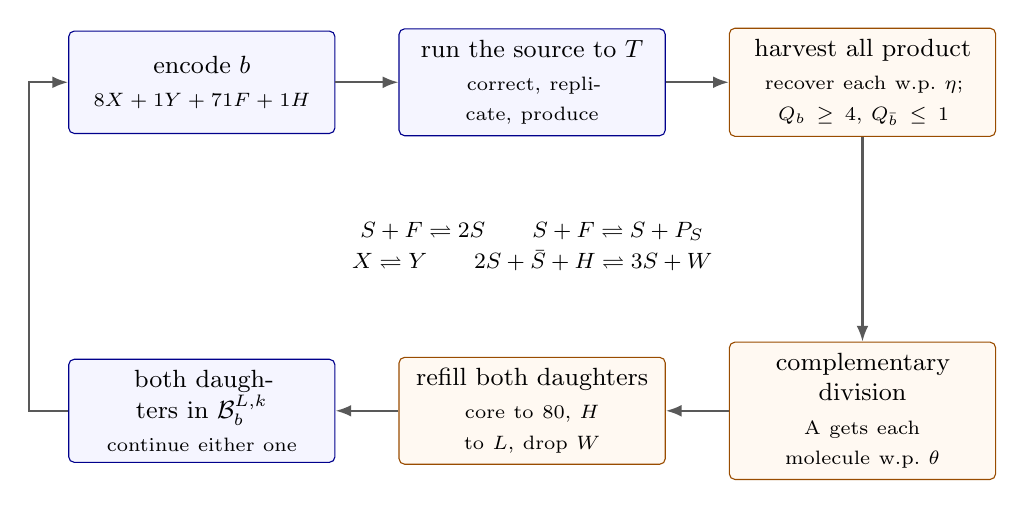
\begin{tikzpicture}[
  font=\small,
  box/.style={draw=blue!55!black,fill=blue!4,rounded corners=2pt,align=center,
              inner sep=4pt,minimum height=13mm,text width=31mm},
  op/.style={draw=orange!60!black,fill=orange!5,rounded corners=2pt,align=center,
             inner sep=4pt,minimum height=13mm,text width=31mm},
  ar/.style={-{Latex[length=2mm]},gray!70!black,thick}]
\node[box] (prep) {encode $b$\\[1pt]{\scriptsize $8X+1Y+71F+1H$}};
\node[box,right=8mm of prep] (run)
  {run the source to $T$\\[1pt]{\scriptsize correct, replicate, produce}};
\node[op,right=8mm of run] (harv)
  {harvest all product\\[1pt]{\scriptsize recover each w.p.\ $\eta$;
   $Q_b\ge4$, $Q_{\bar b}\le1$}};
\node[op,below=26mm of harv] (div)
  {complementary division\\[1pt]{\scriptsize A gets each molecule w.p.\ $\theta$}};
\node[op,left=8mm of div] (refill)
  {refill both daughters\\[1pt]{\scriptsize core to $80$, $H$ to $L$, drop $W$}};
\node[box,left=8mm of refill] (out)
  {both daughters in $\B_b^{L,k}$\\[1pt]{\scriptsize continue either one}};
\draw[ar] (prep) -- (run);
\draw[ar] (run) -- (harv);
\draw[ar] (harv) -- (div);
\draw[ar] (div) -- (refill);
\draw[ar] (refill) -- (out);
\draw[ar] (out.west) -- ++(-5mm,0) |- (prep.west);
\node[align=center,font=\footnotesize] at ($(run.south)!0.5!(refill.north)$)
  {$S+F\rightleftharpoons2S$\qquad $S+F\rightleftharpoons S+P_S$\\[2pt]
   $X\rightleftharpoons Y$\qquad $2S+\bar S+H\rightleftharpoons 3S+W$};
\end{tikzpicture}
\caption{The source and the external batch protocol. Blue: chemistry and the encoded
state. Orange: inventory operations, which are label-blind --- no step reads $b$, and no
resident molecule is supplied, selected or reseeded. The label is used only to state and
score the event \eqref{eq:joint}. This is a mathematical protocol, not a drawing of an
implemented vesicle.}\label{fig:protocol}
\end{figure}

For $i\in\{X,Y\}$ the \emph{joint event} is
\begin{equation}
\mathcal J_i=\bigl\{\,Q_i\ge4,\;\;Q_{\bar i}\le1,\;\;Z_A^+\in\B_i^{L,k},\;\;
Z_B^+\in\B_i^{L,k}\,\bigr\}.\label{eq:joint}
\end{equation}
All four clauses refer to the same trajectory and the same partition. Trajectories
outside $\mathcal J_i$ are failures of a sufficient proof event; they are not removed
from the law, and the process is not conditioned on success at any point.

\subsection{Operating regimes and the main theorem}

\begin{table}[htbp]\centering\footnotesize
\setlength{\tabcolsep}{5pt}
\begin{tabular}{@{}lccccc@{}}\toprule
 & Original & W & O & \textbf{WO} & \textbf{F}\\
 & & wider rates & imperfect ops & both & two minorities\\\midrule
$(L,k)$ & $(1,1)$ & $(1,1)$ & $(1,1)$ & $(1,1)$ & $(64,2)$\\
initial material & $81$ & $81$ & $81$ & $81$ & $144$\\
$\gamma$ & $[10^{9},2\cdot10^{9}]$ & $[2\cdot10^{7},2\cdot10^{9}]$
        & $[10^{8},2\cdot10^{9}]$ & $[2\cdot10^{7},2\cdot10^{9}]$
        & $[2\cdot10^{7},2\cdot10^{9}]$\\
$\beta$ & $[10^{-13},10^{-12}]$ & $[10^{-13},6\cdot10^{-11}]$
        & $[10^{-13},10^{-11}]$ & $[10^{-13},6\cdot10^{-11}]$
        & $[10^{-13},5\cdot10^{-11}]$\\
$\eps$  & $[10^{-10},10^{-9}]$ & $[10^{-10},10^{-7}]$
        & $[10^{-10},10^{-8}]$ & $[10^{-10},10^{-7}]$
        & $[10^{-10},10^{-7}]$\\
$\tau=T-1$ & $10^{-9}$ & $1/(8\cdot10^{7})$ & $1/(4\cdot10^{8})$
        & $1/(8\cdot10^{7})$ & $10^{-7}$\\
$\theta$ & $1/2$ & $1/2$ & $[0.48,0.52]$ & $[0.48,0.52]$ & $[0.48,0.52]$\\
$\eta$ & $1$ & $1$ & $[0.9,1]$ & $[0.9,1]$ & $[0.9,1]$\\\midrule
certified $q$ & $0.9998$ & $0.9998$ & $0.9998$ & $\mathbf{0.9997}$
 & $\mathbf{0.9916}$\\
exact bound & \eqref{eq:qorig} & \eqref{eq:qW} & \eqref{eq:qO} & \eqref{eq:qWO}
 & \eqref{eq:qF}\\\bottomrule
\end{tabular}
\caption{Operating regimes; all coefficients not listed are fixed by
Table~\ref{tab:source}. In each coordinate the box WO is the union of the boxes W and O,
at the cost of one unit in the fourth decimal; the deadline $\tau$ is a protocol choice,
and $\tau=1/(8\cdot10^7)$ is the value forced by the slowest admitted $\gamma$. Regime F
admits two minority molecules and the same imperfect operations. Rates and deadlines are
stated in model units; Section~\ref{sec:physical} discusses their
dimensions.}\label{tab:regimes}
\end{table}

\begin{theorem}[Productive inheritance]\label{thm:main}
For each regime of Table~\ref{tab:regimes}, each $i\in\{X,Y\}$, each $z\in\B_i^{L,k}$ and
every choice of $(\gamma,\beta,\eps,\theta,\eta)$ in the stated intervals,
\begin{equation}
\Prob_z(\mathcal J_i)\;\ge\;q,
\end{equation}
with $q=4999/5000$ in the regimes Original, W and O; $q=9997/10000$ in regime WO; and
$q=2479/2500$ in regime F.
\end{theorem}

Regimes W and O appear separately because their sharper constant $0.9998$ is of
independent interest; regime WO is the statement that one does not have to choose. The
smallest admissible preparations are $(8,1,71,0,0,1,0)$ and its exchange for $k=1$, and
$(8,2,70,0,0,64,0)$ and its exchange for $k=2$. These are absolute-count statements:
scaling the volume and all populations at fixed concentration destroys the one-minority
mechanism, because the falling factorial $y(y-1)$ is not a concentration.

Theorem~\ref{thm:main} is proved in Sections~\ref{sec:core}--\ref{sec:fuel}: the terminal
payoff of a pure core in Proposition~\ref{prop:certificate}, the correction prefix and
the departure hazard in Lemma~\ref{lem:prefix}, the one-minority regimes in
Theorem~\ref{thm:onemin}, and regime F in Theorem~\ref{thm:F}.

\subsection{The logical reading}

Theorem~\ref{thm:main} is a statement about molecule counts. The following two
corollaries say what it means as computation. Fix $k$ and $L$, and define

\begin{itemize}[leftmargin=1.2em]
\item the \emph{compartment decoder} $\mathrm{dec}_{\mathrm c}(z)=i$ if
  $z\in\B_i^{L,k}$, and $\mathrm{dec}_{\mathrm c}(z)=X$ otherwise (any fixed convention
  outside the two regions will do);
\item the \emph{product decoder} $\mathrm{dec}_{\mathrm p}(Q_X,Q_Y)=X$ if $Q_X\ge Q_Y$
  and $Y$ otherwise.
\end{itemize}

\begin{corollary}[Decoded computation]\label{cor:decoder}
In each regime of Table~\ref{tab:regimes}, for every admissible encoding $z$ of $b$,
\begin{equation}
\Prob_z\Bigl(\bigl(\mathrm{dec}_{\mathrm c}(Z_A^+),\,\mathrm{dec}_{\mathrm c}(Z_B^+),\,
\mathrm{dec}_{\mathrm p}(Q_X,Q_Y)\bigr)=(b,b,b)\Bigr)\ \ge\ q .
\end{equation}
Consequently the law of the decoded triple is within total variation $1-q$ of the point
mass at $(b,b,b)$, and each of the three decoded outputs individually equals $b$ with
probability at least $q$.
\end{corollary}

\begin{proof}
On $\mathcal J_b$ the two refilled daughters lie in $\B_b^{L,k}$, so both compartment
decoders return $b$; and $Q_b\ge4>1\ge Q_{\bar b}$, so the product decoder returns $b$.
Thus $\mathcal J_b$ is contained in the event that the triple equals $(b,b,b)$, and
Theorem~\ref{thm:main} applies. A bound on the probability that a random variable differs
from a constant bounds the total variation distance to the point mass at that constant.
\end{proof}

The joint statement is strictly stronger than the three marginal statements, because the
three outputs are produced by one trajectory and one partition and are certainly not
independent. Note also what the corollary does \emph{not} say: it is a total-variation
bound on \emph{decoded} outputs, not a claim that the microscopic terminal distribution
is close to a single ideal chemical state.

\begin{corollary}[Information per batch]\label{cor:fano}
Let $B$ be a uniformly random input bit, encoded by any admissible state of
$\B_B^{L,k}$, and let $D$ be any one of the three decoded outputs of
Corollary~\ref{cor:decoder}. Then, with $h_2$ the binary entropy in bits,
\begin{equation}
I(B;D)\ \ge\ 1-h_2(1-q).
\end{equation}
Numerically this is at least $0.997254$ bits in regimes W and O, $0.996056$ bits in
regime WO and $0.930011$ bits in regime F.
\end{corollary}

\begin{proof}
$\Prob[D\ne B]\le 1-q\le 1/2$, so Fano's inequality for a binary variable gives
$H(B\mid D)\le h_2(\Prob[D\ne B])\le h_2(1-q)$, and $I(B;D)=1-H(B\mid D)$.
\end{proof}

This is an information-theoretic reading of an existing bound, not a channel-coding
theorem and not a measured rate: it counts neither the time nor the material cost of the
measurement, both of which are outside the modelled inventory.

\section{The finite core and its exact lower certificate}\label{sec:core}

Suppress leakage and correction, and restrict the state to one pure resident face. With
resident count $n$, selected-product stock $p$ and food $f=80-n-p$, the four surviving
propensities are
\begin{equation}
\underbrace{nf}_{\text{replicate}},\quad \underbrace{n(n-1)/100}_{\text{reverse}},\quad
\underbrace{nf}_{\text{produce}},\quad \underbrace{np/100}_{\text{reverse}} .
\label{eq:core}
\end{equation}
The states $1\le n\le 80$, $0\le p\le 80-n$ number $3\,240$. Let $G$ be the row generator
of this core chain acting on column payoff vectors. The terminal payoff of the protocol
is
\begin{equation}
H_{\theta,\eta}(n,p)=a_p(\eta)\,g_n(\theta),\qquad
a_p(\eta)=\Prob\{\Bin(p,\eta)\ge4\},\qquad
g_n(\theta)=\Prob\{8\le\Bin(n,\theta)\le n-8\}.\label{eq:payoff}
\end{equation}
Two modelling points are built into \eqref{eq:payoff}. First, $g_n$ uses \emph{one}
binomial draw: if daughter A receives $J$ residents then B receives $n-J$, so requiring
$8\le J\le n-8$ is exactly the requirement that both daughters are admissible. Second,
$a_p$ is evaluated at the \emph{terminal stock} $p$, not at the number of forward
production events: the production reaction is reversible and its reverse consumes
product. The one-unit joint probability from a core state is $(e^{G}H_{\theta,\eta})$
evaluated there.

\begin{lemma}[Endpoint reduction]\label{lem:endpoint}
For all $\theta\in[0.48,0.52]$ and $\eta\in[0.9,1]$ and every state $(n,p)$,
\[
H_{\theta,\eta}(n,p)\ \ge\ H_{0.48,0.9}(n,p).
\]
\end{lemma}

\begin{proof}
A binomial count is stochastically nondecreasing in its success parameter (couple all
trials to a common uniform vector), so $a_p(\eta)\ge a_p(0.9)$ for $\eta\ge0.9$; and
$a_p\ge0$, $g_n\ge0$, so it suffices to treat the two factors separately. For $n<16$ we
have $g_n\equiv0$. For $n\ge16$, differentiating the $j$th binomial mass
$\binom nj\theta^j(1-\theta)^{n-j}$ gives $n$ times the difference of the $(j-1)$st and
$j$th masses for $n-1$ trials, so the sum defining $g_n$ telescopes to
\begin{equation}
g_n'(\theta)=n\binom{n-1}{7}\theta^{7}(1-\theta)^{7}
\bigl((1-\theta)^{\,n-15}-\theta^{\,n-15}\bigr).\label{eq:derivative}
\end{equation}
The bracket is nonnegative for $\theta\le1/2$ and nonpositive for $\theta\ge1/2$, so
$g_n$ increases up to $1/2$ and decreases after it. Since $g_n(\theta)=g_n(1-\theta)$, we
get $g_n(0.52)=g_n(0.48)$ and hence $\min_{[0.48,0.52]}g_n=g_n(0.48)$.
\end{proof}

Lemma~\ref{lem:endpoint} is what makes a statement about a continuum of operation
parameters provable by a finite computation: it is an analytic reduction to one endpoint,
not a scan over a grid of parameter values. (The sign of \eqref{eq:derivative} on the left
half-interval and the monotonicity of the product are machine-checked; the telescoping
identity itself is a conventional step.)

\begin{proposition}[Exact core certificate]\label{prop:certificate}
Uniformly over every pure newborn $(n,0)$ with $8\le n\le80$,
\begin{align}
\bigl(e^{G}H_{1/2,1}\bigr)(n,0)&\ \ge\ c:=\frac{2147232289}{2147483648},\label{eq:c}\\
\bigl(e^{G}H_{0.48,0.9}\bigr)(n,0)&\ \ge\ c_{\mathrm O}:=\frac{2147153442}{2147483648}.
\label{eq:co}
\end{align}
Both minima are attained at $n=8$; the range includes $n=80$, for which the newborn has
no food at all.
\end{proposition}

\begin{proof}[Certificate and its soundness]
All four rates in \eqref{eq:core} are integer multiples of $1/100$, and the total exit
rate is bounded by $\lambda=3216$ (Lemma~\ref{lem:prefix} proves the sharper
$3215.6$). Put $P=I+G/\lambda=A/D$ with $D=100\lambda=321600$; then $A$ is a nonnegative
integer matrix and every row of $A$ sums to $D$, so $P$ is a stochastic matrix and the
uniformization identity $e^{G}=e^{-\lambda}\sum_{j\ge0}(\lambda P)^j/j!$
holds~\citep{jensen1953,grassmann1977}. Let $S=2^{31}$ and
\begin{equation}
e_-:=\sum_{m=0}^{25}\frac{(-1)^m}{m!}<e^{-1},\qquad
w_j:=\Bigl\lfloor \frac{S\,e_-}{j!}\Bigr\rfloor\quad(0\le j\le 18),\label{eq:weights}
\end{equation}
where the strict inequality is the alternating-series remainder estimate. All $w_j$ are
nonnegative and $w_j=0$ for $j>12$ at this scale. For an integer vector $0\le v\le S$
define
\begin{equation}
v^{[0]}=v,\qquad v^{[j+1]}=\bigl\lfloor Av^{[j]}/D\bigr\rfloor,\qquad
\mathcal D(v)=\Bigl\lfloor \frac{\sum_{j=0}^{18}w_jv^{[j]}}{S}\Bigr\rfloor,
\label{eq:round}
\end{equation}
all roundings coordinatewise and downward. Since $A$ is nonnegative, induction gives
$v^{[j]}/S\le P^{j}(v/S)$ coordinatewise, and therefore
\begin{equation}
\mathcal D(v)/S\ \le\ \sum_{j\ge0}\frac{e^{-1}}{j!}P^{j}(v/S)=e^{G/\lambda}(v/S),
\end{equation}
where dropping the terms with $j>18$ is legitimate because every omitted term is
nonnegative. Start from $v=\lfloor S\,H_{\theta,\eta}\rfloor\le S\,H_{\theta,\eta}$ and
apply $\mathcal D$ exactly $\lambda=3216$ times. The Markov semigroup is monotone, so
composing the $3216$ blocks gives $\mathcal D^{3216}(v)/S\le e^{G}H_{\theta,\eta}$
coordinatewise. Taking the minimum over the $73$ newborn coordinates $(n,0)$,
$8\le n\le 80$, yields \eqref{eq:c} and \eqref{eq:co}.

The implementation is exact in signed $64$-bit arithmetic: the largest matrix
accumulator is bounded by $DS=690630741196800<2^{63}$ and the largest weighted sum by
$S\sum_j w_j=4611686007689969664<2^{63}$; every summand is nonnegative and the invariant
$0\le v_i\le S$ is preserved, so the bounds control partial sums as well. No
floating-point matrix exponential enters at any stage. The complete state enumeration,
the row sums, the outgoing transitions and the minimum are recomputed by the supplied
scripts; this execution is exact-computation evidence, and Appendix~\ref{app:evidence}
states exactly which parts of the argument are additionally kernel-checked.
\end{proof}

\begin{remark}
The rounding is deliberately one-sided in the safe direction, and the resulting slack is
small: at $(8,0)$ with ideal operations the certified value \eqref{eq:c} is
$0.99988295\ldots$ against an unrounded double-precision evaluation of $0.99989142\ldots$,
so the certificate costs about $8.5\cdot10^{-6}$ of the error budget. Increasing the core
inventory tightens the payoff quickly --- the same computation at $K=64$ gives only
$0.997547\ldots$ and at $K=96$ gives $0.999983\ldots$ --- which is why the core is fixed at
$80$ resident-plus-product units.
\end{remark}

\section{A fixed-time coupling for one-minority correction}\label{sec:coupling}

The comparison chains in this section are proof devices only. The physical source of
Table~\ref{tab:source} runs unchanged throughout the batch; we never switch rates at a
random time and never condition on a stopping time.

\begin{lemma}[Prefix and departure bounds]\label{lem:prefix}
Consider the \emph{repair-only} chain obtained from Table~\ref{tab:source} by retaining
only the two forward correction reactions. Along it, the total propensity of all
suppressed channels is at most
\begin{equation}
2r(80-r)+\frac{r(r-1)}{100}\ \le\ \frac{16078}{5}=3215.6\qquad (8\le r\le 80),
\label{eq:prefixmax}
\end{equation}
where $r=x+y$, and therefore at most $B=3216$ in the regimes W, O, WO and F. On a pure
face carrying $k$ spent fuel units, leakage and reverse correction have total propensity
at most
\begin{equation}
80\eps+80^{3}\beta k .\label{eq:departure}
\end{equation}
\end{lemma}

\begin{proof}
The repair-only chain preserves $r$ and creates no product, so $f=80-r$ throughout and
$p=0$. The suppressed channels are forward replication and forward production, each of
total propensity $rf=r(80-r)$, their reverses, of total propensity at most
$r(r-1)/100$ and $0$ respectively, leakage, of propensity $\eps r\le80\eps$, and reverse
correction, of propensity at most $\beta L\,(\ff x3+\ff y3)\le\beta L\,80^3$ --- using
$\ff x3+\ff y3\le(x+y)^3$. For the polynomial part, multiplying the claimed deficit by
$100$ gives $16078/5-2r(80-r)-r(r-1)/100\ge0 \iff (r-40)(199r-8039)\ge0$, which holds for
every integer $r$ because the two factors change sign between $r=40$ and $r=41$; the
maximum $3215.6$ is attained at $r=40$. The largest rare-channel allowance used in this
paper is that of regime F, namely $80\cdot10^{-7}+64\cdot80^{3}\cdot5\cdot10^{-11}
=1.6464\cdot10^{-3}$, well inside the remaining $0.4$; regime WO needs
$80\cdot10^{-7}+80^{3}\cdot6\cdot10^{-11}=3.872\cdot10^{-5}$. On a pure face both forward
correction propensities vanish (each requires a molecule of each label), the product
stock contributes only its own reverse, and the spent fuel is $w=k$, which gives
\eqref{eq:departure}.
\end{proof}

\begin{theorem}[One-minority regimes]\label{thm:onemin}
Let $k=1$, $L=1$, and let $c_*$ denote $c$ under ideal operations and $c_{\mathrm O}$ for
$\theta\in[0.48,0.52]$, $\eta\in[0.9,1]$. Then for every $z\in\B_i^{1,1}$,
\begin{equation}
\Prob_z(\mathcal J_i)\ \ge\ c_*-e^{-56\gamma\tau}-B\tau-80\eps-80^{3}\beta .
\label{eq:onebound}
\end{equation}
In particular
\begin{align}
q_{\mathrm{Orig}}&\ \ge\ c-\tfrac{15}{10^{6}}
 =\tfrac{6710000239829}{6710886400000}>\tfrac{4999}{5000},\label{eq:qorig}\\
q_{\mathrm W}&\ \ge\ c-\tfrac{999}{12500000}
 =\tfrac{838695571135489}{838860800000000}>\tfrac{4999}{5000},\label{eq:qW}\\
q_{\mathrm O}&\ \ge\ c_{\mathrm O}-\tfrac{187}{12500000}
 =\tfrac{419359631961841}{419430400000000}>\tfrac{4999}{5000},\label{eq:qO}\\
q_{\mathrm{WO}}&\ \ge\ c_{\mathrm O}-\tfrac{999}{12500000}
 =\tfrac{419332385763057}{419430400000000}>\tfrac{9997}{10000}.\label{eq:qWO}
\end{align}
\end{theorem}

\begin{proof}
Fix $z\in\B_i^{1,1}$ and suppose first $y=1$. Because $y(y-1)=0$, the \emph{opposing}
forward correction reaction has propensity zero, while the selected one has propensity
$\gamma h\,x(x-1)y=\gamma x(x-1)\ge56\gamma$ for $x\ge8$ and $h=1$. In the repair-only
chain a single event therefore converts the minority, leaving a pure state with
$x'=x+1\in[9,80]$, $p=0$, $w=1$, and the chain then stops. Hence the repair-only chain
fails to complete by $\tau$ with probability exactly $e^{-\gamma x(x-1)\tau}\le
e^{-56\gamma\tau}$. If $y=0$ no repair is needed and this term is absent.

Couple the literal source to the repair-only chain on $[0,\tau]$ by common reaction
clocks: run the same Poisson clocks and let the literal chain follow the comparison chain
until the first firing of a suppressed clock. The two agree unless some suppressed clock
fires, and the probability of that is at most the expected integrated suppressed
propensity, which by \eqref{eq:prefixmax} is at most $B\tau$. On the complementary event
and on completion of the repair, the literal state at the \emph{fixed} time $\tau$ is a
pure newborn $(n,0)$ with $8\le n\le80$ and $w\le1$.

Apply the Markov property at the deterministic time $\tau$. On $[\tau,\tau+1]$ couple the
literal source to the pure core \eqref{eq:core} by the same device; the only channels
present in the literal source and absent from the core are leakage and reverse
correction, whose total propensity is bounded by \eqref{eq:departure} with $k\le1$, so
the two agree over one time unit except on an event of probability at most
$80\eps+80^3\beta$. On agreement, the terminal payoff of the core is at least $c_*$ by
Proposition~\ref{prop:certificate} and Lemma~\ref{lem:endpoint}, and by construction the
payoff \eqref{eq:payoff} is exactly the probability that $Q_i\ge4$, $Q_{\bar i}=0$ and
both refilled daughters lie in $\B_i^{1,1}$. Subtracting the three error events gives
\eqref{eq:onebound}. No independence between the error events is used; they are removed
by a union bound.

For the numerical instances: in regimes W, O and WO the minimal repair exponent is
$56\gamma_{\min}\tau=14$, and the finite rational inequality
$\sum_{j=0}^{18}14^{j}/j!>10^{6}$ certifies $e^{-14}<10^{-6}$. The remaining terms are
$B\tau$, $80\eps_{\max}$ and $80^3\beta_{\max}$, evaluated at the endpoints of each box,
which are the worst cases because \eqref{eq:onebound} is monotone in each of them. The
original regime uses exponent $56$ and the conservative total loss $15/10^{6}$.
\end{proof}

\begin{figure}[htbp]\centering

\includegraphics[width=\linewidth]{certificate.pdf}
\caption{Left: the exact core certificate as a function of the partition probability at
recovery $0.9$. The theorem uses only the endpoint $\theta=0.48$ together with
Lemma~\ref{lem:endpoint}; the other two points are comparisons, not a proof by scanning.
Right: the four terms of the certified error budget in regimes WO and F, on a logarithmic
scale. In both regimes the cost of the partition and output requirement dominates; the
repair deadline, which is the term that the extreme rate constants buy, is the
smallest.}\label{fig:certificate}
\end{figure}

\begin{remark}[The certificate frontier]\label{rem:frontier}
The same argument proves a family statement. For core inventory $K$, minimum residents
per daughter $m$, pure-core certificate $c$, correction rate lower bound
$a=m(m-1)\gamma$, suppressed prefix bound $B$ and core horizon $t$,
\begin{equation}
\Prob_z(\mathcal J_i)\ \ge\ c-e^{-a\tau}-B\tau-\bigl(K\eps+K^{3}\beta\bigr)t .
\label{eq:frontier}
\end{equation}
The first two terms compete. For fixed $B<a$ the sum $e^{-a\tau}+B\tau$ is minimised at
$\tau_\ast=a^{-1}\log(a/B)$, with value $(B/a)\bigl(1+\log(a/B)\bigr)$; for $a\le B$ it
is minimised at $\tau=0$, and this proof architecture then cannot give a small loss at
all. At the regime WO values $a=1.12\cdot10^{9}$ and $B=3216$ the optimum is
$\tau_\ast=1.139\cdot10^{-8}$ with value $3.95\cdot10^{-5}$; our rational choice
$\tau=1/(8\cdot10^{7})$ gives $4.10\cdot10^{-5}$, so nothing material is lost by
preferring a transparent deadline. The visible consequence of \eqref{eq:frontier} is that
high fidelity here is bought with \emph{kinetic separation}, $a\gg B$, and that a protocol
which lowered $B$ --- for instance by withholding production food until a fixed
repair interval has elapsed --- would relax the demand on $a$ by the same factor. Such a
staged protocol is a different model and would need its own proof; we do not claim it
here.
\end{remark}

\section{Finite fuel, wrong consensus and spent inventory}\label{sec:fuel}

\subsection{The embedded correction chain}

Let $r=x+y\ge3$ be the resident total and let $j$ count $Y$ residents. In the repair-only
chain the two correction propensities are
\begin{equation}
\text{down}:\ \gamma h\,(r-j)(r-j-1)j,\qquad
\text{up}:\ \gamma h\,j(j-1)(r-j).
\end{equation}
Their sum is $\gamma h\,j(r-j)(r-2)$, so for $0<j<r$ and $h>0$ the embedded jump chain
has
\begin{equation}
p_-(j)=\frac{r-j-1}{r-2},\qquad p_+(j)=\frac{j-1}{r-2}.\label{eq:walk}
\end{equation}
The common factor $\gamma h$ cancels: \emph{the direction of correction does not depend on
the catalytic rate constant, on the amount of fuel remaining, or on time}. Each jump
spends one $H$ and creates one $W$. (The factorisation and the normalised jump
probability are machine-checked.)

\begin{theorem}[Consensus law]\label{thm:walk}
For the embedded chain with unlimited steps, the probability $u_r(j)$ of reaching $r$
before $0$ is
\begin{equation}
u_r(j)=2^{-(r-3)}\sum_{a=0}^{j-2}\binom{r-3}{a}\quad(1\le j\le r-1),\qquad
u_r(0)=0,\quad u_r(r)=1,\label{eq:consensus}
\end{equation}
the empty sum being zero. For a fuel inventory $L$, the probability $v_L(j)$ of reaching
$0$ within $L$ jumps satisfies
\begin{equation}
v_0(j)=\ind_{\{j=0\}},\quad v_L(0)=1,\quad v_L(r)=0,\qquad
v_L(j)=p_-(j)v_{L-1}(j-1)+p_+(j)v_{L-1}(j+1).\label{eq:fuelrec}
\end{equation}
\end{theorem}

\begin{proof}
States $1$ and $r-1$ can leave only towards $0$ and $r$ respectively, since $p_+(1)=0$
and $p_-(r-1)=0$; so $u_r(1)=0$ and $u_r(r-1)=1$. Every interior state has a positive
finite path to an endpoint, and the state space is finite, so absorption is almost sure
and $u_r$ is the unique bounded harmonic function with these boundary values. Writing
$d_j=u_r(j)-u_r(j-1)$, harmonicity gives $d_{j+1}=\frac{r-j-1}{j-1}d_j$ for
$2\le j\le r-2$, whence $d_j=d_2\binom{r-3}{j-2}$, and summing all differences to $1$
gives $d_2=2^{-(r-3)}$. This is \eqref{eq:consensus}. First-step conditioning with
absorbing boundary values gives \eqref{eq:fuelrec}.
\end{proof}

\begin{remark}[Provenance]\label{rem:mabinogion}
Substituting $N=r-2$ and $\kappa=j-1$ turns \eqref{eq:walk} into ``increase with
probability $\kappa/N$'': the embedded chain is the Mabinogion urn, whose absorption
probability was computed in closed form by \citet{flajolet2008} in an equivalent integral
form, and studied further by \citet{huillet2009} and \citet{stenlund2018}. The
tri-molecular majority network itself is that of \citet{condon2020}, who record the
embedded jump probability and then bound it in order to obtain Chernoff-type consensus
estimates for large populations with a large initial gap; they do not use an exact
absorption probability, which is what a small-count guarantee needs. So
\eqref{eq:consensus} should be read as the urn law transported to this network, not as a
new identity. What is new here is everything that follows from running the chain with a
\emph{finite} fuel inventory: the truncation \eqref{eq:fuelrec}, the joint absorption/
spent-fuel law of \S\ref{sec:spent}, and its use as a source-level transfer.
\end{remark}

\begin{corollary}[Inventory rule for the correction step]\label{cor:inventory}
From exactly two minority molecules, $u_r(2)=2^{-(r-3)}$. Hence the correction step alone
achieves wrong-consensus probability at most $\delta$, even with unlimited fuel and
unlimited speed, if and only if
\begin{equation}
r\ \ge\ 3+\bigl\lceil\log_2(1/\delta)\bigr\rceil .
\end{equation}
For $\delta=2\cdot10^{-4}$ this forces $r\ge16$; at $r=16$ the wrong-consensus
probability is $1/8192$, leaving only $7.79\cdot10^{-5}$ of the budget for every other
failure mode.
\end{corollary}

This is the quantitative reason why regime F cannot simply inherit the $0.9998$ headline
of the one-minority regimes: at its smallest admitted state, $r=10$, the floor is
$1/128$. It also explains why the fix is not ``more fuel'' and not ``larger $\gamma$'',
but \emph{more residents}; and since the restart region \eqref{eq:restart} demands at
least $8$ residents in each daughter, raising the residents required at restart would
also raise the partition threshold, which is a different trade-off from the one this
corollary describes. The corollary is about one subproblem of the contract; it is not an
asymptotic inventory bound for the whole module.

\begin{figure}[htbp]\centering

\includegraphics[width=\linewidth]{fuel.pdf}
\caption{Left: exact correct-consensus probabilities from two minority molecules as a
function of the available fuel, by the recursion \eqref{eq:fuelrec}; the dotted lines are
the unlimited-fuel limits of Theorem~\ref{thm:walk}. More fuel removes the exhaustion
loss but cannot remove the wrong-consensus floor at a fixed resident total. Right: the
floor $u_r(2)=2^{-(r-3)}$ against the target $\delta=2\cdot10^{-4}$, i.e.\
Corollary~\ref{cor:inventory}.}\label{fig:fuel}
\end{figure}

\subsection{Charging the fuel that is actually spent}\label{sec:spent}

Let $a_{r,j}(k,b)$ be the probability that the embedded chain started at $j$ is first
absorbed at endpoint $b\in\{0,r\}$ on jump $k\le L$. Propagating the transient mass by
\eqref{eq:walk} and removing newly absorbed mass to a table costs $O(rL)$ rational
operations. Put
\begin{equation}
v_b=\sum_{k=0}^{L}a_{r,j}(k,b),\qquad s_b=\sum_{k=0}^{L}k\,a_{r,j}(k,b),\label{eq:spent}
\end{equation}
so that $v_b$ is the absorption mass and $s_b$ is the \emph{unnormalised} first moment of
the fuel spent on that event; $s_b/v_b$ is the conditional mean when $v_b>0$. Transient
mass is retained, so absorbed plus transient mass is exactly one at every step.

\begin{lemma}[Fuel-sensitive source comparison]\label{lem:spent}
Suppose the repair-only chain fails to be absorbed by the deadline $\tau$ with probability
at most $d$, the suppressed prefix propensity is at most $B$, and the pure-core
certificate is $c_*$. Then the probability of productive return to the program
represented by endpoint $b$ is at least
\begin{equation}
(c_*-80\eps)\,v_b-80^{3}\beta\,s_b-B\tau-d .\label{eq:spentbound}
\end{equation}
\end{lemma}

\begin{proof}
On the event that absorption occurs at $b$ after exactly $k$ jumps and before $\tau$, the
compartment at time $\tau$ is a pure newborn carrying $w=k$ spent fuel units, so by
Lemma~\ref{lem:prefix} the departure hazard over the subsequent unit interval is at most
$80\eps+80^3\beta k$ and the conditional probability of the joint event is at least
$c_*-80\eps-80^3\beta k$ by the argument of Theorem~\ref{thm:onemin}. Summing this
conditional bound against the absorption table gives
$\sum_k a_{r,j}(k,b)\,(c_*-80\eps-80^3\beta k)=(c_*-80\eps)v_b-80^3\beta s_b$. Paths not
absorbed by $\tau$ are discarded at cost at most $d$, since a terminal probability is at
most one; the omitted suppressed clocks cost at most $B\tau$ as before; and the Markov
property is applied at the fixed time $\tau$.
\end{proof}

The point of \eqref{eq:spentbound} is that it keeps the \emph{dependence} between how the
correction ended and how much fuel it burned. The coarse alternative --- charging
$w=L$ on every successful path, because $L$ units were available --- is what the previous
version of this construction did, and it costs an order of magnitude in the final bound
(Remark~\ref{rem:sharp}). Spent fuel is the state statistic that controls the downstream
hazard, and it must be carried.

\begin{theorem}[Two minority molecules]\label{thm:F}
In regime F, uniformly over $\B_i^{64,2}$ and the stated parameter intervals,
$\Prob_z(\mathcal J_i)\ge q_{\mathrm F}$ where
\begin{equation}
q_{\mathrm F}=\frac{176915425816575482750126908089960417712372422485900866047}
{178405961588244985132285746181186892047843328000000000000}
\;>\;\frac{2479}{2500}.\label{eq:qF}
\end{equation}
Its decimal expansion is $0.9916452580485533\ldots$; with ideal operations
($\theta=1/2$, $\eta=1$) the same argument gives $0.9916816872003354\ldots$.
\end{theorem}

\begin{proof}
Every state of the restart region has $r-j\ge8$ and $j\le2$, hence $r\ge8$ and, when
$j=2$, $r\ge10$. While fuel remains, the total correction propensity from a transient
state is $\gamma h\,j(r-j)(r-2)\ge \gamma\cdot1\cdot(r-2)\cdot(r-j)\ge72\gamma$ for
$r\ge10$, $j=2$. At most $L=64$ jumps can occur before the fuel is exhausted, so the time
to absorption or exhaustion is stochastically dominated by a sum of $64$ exponentials of
rate $72\gamma\ge72\cdot2\cdot10^{7}$; with $\tau=10^{-7}$ the exponent is
$72\cdot2\cdot10^{7}\cdot10^{-7}=144$ and
\begin{equation}
d\ \le\ e^{-144}\sum_{m=0}^{63}\frac{144^{m}}{m!}\ <\ 10^{-12},\label{eq:clock64}
\end{equation}
which we verify exactly by dividing the numerator polynomial by the lower Taylor sum
$\sum_{m=0}^{300}144^{m}/m!\le e^{144}$; the resulting rational bound is below
$2.44\cdot10^{-14}$. A start with $j=1$ needs one jump with exponent at least $7168$, and
a start with $j=0$ needs none, so the same allowance $d=10^{-12}$ is valid on the whole
restart region.

Now apply Lemma~\ref{lem:spent} with $c_*=c_{\mathrm O}$ (legitimate for the whole
operation box by Lemma~\ref{lem:endpoint}), $\eps=10^{-7}$, $\beta=5\cdot10^{-11}$,
$B=3216$, $\tau=10^{-7}$ and $b=0$, evaluated by exact rational arithmetic at each of the
$216$ admissible pairs $(r,j)$ with $j\le 2$ and $r-j\ge8$. Every value exceeds
$2479/2500$, and the minimum is attained at $(r,j)=(10,2)$, giving \eqref{eq:qF}. At that
state $v_0=0.992187499369\ldots$ and the conditional mean fuel expenditure is
$s_0/v_0=2.36775398866\ldots$, far below the $64$ units available. Successful daughters
are pure and lie in the larger region $\B_i^{64,2}$.
\end{proof}

\begin{remark}[Sharpness]\label{rem:sharp}
The bound \eqref{eq:qF} is close to the best possible for this correction mechanism.
Theorem~\ref{thm:walk} gives the ceiling $1-u_{10}(2)=127/128=0.9921875$ for the worst
admitted state, even with unlimited fuel and unlimited catalytic speed; the exact
$64$-jump truncation reaches $0.9921874993\ldots$, within $6.4\cdot10^{-10}$ of it, and
the certified source bound \eqref{eq:qF} is within $5.5\cdot10^{-4}$ of it. In other
words, of the $8.35\cdot10^{-3}$ failure allowance in regime F, $7.81\cdot10^{-3}$ is the
irreducible wrong-consensus floor of the majority mechanism at $r=10$ and only
$5.5\cdot10^{-4}$ is the cost of everything else the theorem covers: the exhaustion of
fuel, the terminal partition and output requirement, the clock couplings, the leakage and
the reverse correction. For comparison, charging every successful path the full $64$ fuel
units --- because $64$ were available --- gives only $0.9900657\ldots$, i.e.\ it loses a
further $1.58\cdot10^{-3}$, nearly three times the entire remaining budget.
\end{remark}

\section{Heritable variation and its state dependence}\label{sec:variation}

The same absorption table that certifies correct inheritance also certifies its failure
mode, and the failure mode is heritable: the opposite endpoint of the correction chain is
a compartment running the \emph{other} program, which then makes the other product and
transmits the other program to both of its daughters.

\begin{corollary}[A productive program switch]\label{cor:flip}
In regime F, from the specified mixed preparation $(8,2,70,0,0,64,0)\in\B_X^{64,2}$, the
probability that $Q_Y\ge4$, $Q_X\le1$ and both refilled daughters lie in $\B_Y^{64,2}$ is
greater than $37/5000=0.0074$.
\end{corollary}

\begin{proof}
Apply Lemma~\ref{lem:spent} with the same constants and $b=r=10$. Exact recursion gives
$v_{10}=5316911553929185963121618191138170975/680564733841876926926749214863536422912$
and $s_{10}/v_{10}=11.3714239539\ldots$, and \eqref{eq:spentbound} evaluates to
$0.00748736130\ldots>37/5000$. The daughter and product clauses come from the pure-core
certificate on the \emph{opposite} face, so this is a fully productive opposite-program
pair, not a transient leakage event.
\end{proof}

For $128$ independent founders of this preparation, the probability that at least one
productive opposite pair appears is at least $1-(1-37/5000)^{128}>0.6135>1/2$.
Independence of founders is an extra protocol assumption, used only here and not in
Theorem~\ref{thm:main}.

Corollary~\ref{cor:flip} is a statement about a mixed preparation. The next theorem shows
that it cannot be reinterpreted as a per-generation mutation rate, because a pure newborn
behaves entirely differently --- and it does so for a structural reason that is visible in
the reaction table.

\begin{theorem}[Pure-start obstruction]\label{thm:pure}
Let $z$ be a pure newborn: $y=0$, $p_X=p_Y=0$, $h=L$, $w=0$ (any state of
$\B_X^{L,k}$ with no minority). Then, up to the first time a molecule of $Y$ appears:
\begin{enumerate}[label=(\roman*),leftmargin=2.2em]
\item both forward correction reactions have propensity zero, since each requires a
  molecule of each label;
\item both reverse correction reactions have propensity zero, since each requires $w\ge1$
  and $W$ can be created only by a forward correction reaction;
\item no other reaction creates $Y$ or $W$.
\end{enumerate}
Consequently the only channel that can create the first minority molecule is the leakage
$X\to Y$, whose propensity is $\eps x\le 80\eps$, and for any deadline $T$,
\begin{equation}
\Prob_z(\text{a productive opposite-program daughter pair by }T)\ \le\
1-e^{-80\eps T}\ \le\ 80\eps T .\label{eq:purebound}
\end{equation}
In regime F, with $\eps\le10^{-7}$ and $T=1+10^{-7}$, the right-hand side is
$8.0000008\cdot10^{-6}<8.1\cdot10^{-6}$.
\end{theorem}

\begin{proof}
Items (i)--(iii) are read off Table~\ref{tab:source}: the forward correction reactions
have propensities $\gamma h\,x(x-1)y$ and $\gamma h\,y(y-1)x$, both zero when $y=0$; the
reverse ones carry the factor $w$, and the only reactions producing $W$ are the forward
correction reactions, which are disabled; and replication, production and their reverses
change only $x,f,p_X$. Hence $w=0$ and $y=0$ persist until the leakage clock fires. A
productive opposite-program pair requires $Q_Y\ge4$, which requires at least one molecule
of $P_Y$, which requires at least one molecule of $Y$ at some time. The first such
molecule must be created by leakage, whose propensity is at most $80\eps$ while it is
disabled elsewhere, so the probability that it fires before $T$ is at most
$1-e^{-80\eps T}$, and $1-e^{-u}\le u$.
\end{proof}

\begin{corollary}[No label-only switching kernel]\label{cor:nokernel}
In regime F the mixed preparation of Corollary~\ref{cor:flip} produces a productive
opposite-program pair with probability greater than $0.0074$, while a pure newborn of the
same region does so with probability at most $8.1\cdot10^{-6}$ --- a factor above $935$.
No Markov kernel on the two-element label set $\{X,Y\}$ can therefore describe the
one-cycle offspring law of this source uniformly over its restart region. A population
model must retain at least the minority count, or must use region-dependent bounds.
\end{corollary}

Theorem~\ref{thm:pure} improves by a factor of $205.8$ the bound we can obtain by
charging, in addition to leakage, the reverse correction channel at its maximal rate
$64\cdot80^{3}\beta$; that channel is simply not available to a newborn that has not yet
made any waste. It is an upper bound, so it does \emph{not} prove that recurrent mutation
is zero: a positive lower bound on the switching probability from the actual distribution
of pure descendants remains open, and is the missing ingredient for any statement about
sustained adaptation. We regard identifying the missing state variable as the useful
content of this section.

\begin{figure}[htbp]\centering

\includegraphics[width=\linewidth]{variation.pdf}
\caption{Left: the certified two-sided gap of Corollary~\ref{cor:nokernel}. The two bars
are bounds of opposite sense --- a lower bound for the mixed preparation, an upper bound
for the pure newborn --- so the separation is a theorem, not an estimate. Right: intact
clusters change the partition law even at equal total moiety count
(Proposition~\ref{prop:cluster}); $32$ resident moieties carried by free monomers, dimers
or tetramers fail the ``at least $8$ in each daughter'' test with very different
probabilities.}\label{fig:variation}
\end{figure}

\section{Iteration, material and external selection}\label{sec:selection}

\begin{corollary}[A preselected lineage]\label{cor:lineage}
Fix a regime and designate daughter A, in advance of the partition, as the one that
continues. For $m$ inspected divisions the probability that all $m$ joint events occur is
at least $q^{m}$, and at least $4m$ selected product molecules are collected on that
event. In particular ten divisions succeed jointly with probability greater than
$0.998$ in regimes W and O, greater than $0.997$ in regime WO, and greater than $0.919$
in regime F.
\end{corollary}

\begin{proof}
Every successful continued daughter lies in the same restart region, over which
Theorem~\ref{thm:main} is uniform. Hence, conditional on any prior successful history, the
next joint event has probability at least $q$; repeated conditioning gives $q^m$. No
independence of cycles is assumed. Both daughters are checked at each division of this
lineage; the statement is not about an exponentially growing family tree. (For a
scheduled family tree with at most $N$ divisions, all of them operated by the same
protocol, a union bound gives failure at most $N(1-q)$; note that a complete binary tree
of depth $d$ has $2^{d}-1$ divisions, not $d$.)
\end{proof}

If the terminal product stock is $p=p_X+p_Y$, the two daughter cores together hold
$80-p$ residents and food after harvesting, so refilling both to $80$ supplies exactly
$80+p\le160$ units of $F$. Fuel supplied is at most $2L$ and waste removal at most $L$
per division. Table~\ref{tab:resources} collects the bill, including material that
selection later discards.

\begin{table}[htbp]\centering\small
\begin{tabular}{@{}lrr@{}}\toprule
Quantity (modelled material units) & One-minority regimes & Regime F\\\midrule
Initial material per compartment & $81$ & $144$\\
Maximum resident moieties & $80$ & $80$\\
Food supplied per division, both daughters & $\le160$ & $\le160$\\
Fuel supplied per division, both daughters & $\le2$ & $\le128$\\
Waste fuel removed per division & $\le1$ & $\le64$\\
Unrecovered product discarded (imperfect recovery) & $\le80$ & $\le80$\\
Initial plus ten divisions of one lineage & $\le1701$ & $\le3024$\\
Initial plus one division for $20$ founders & $\le4860$ & $\le8640$\\\bottomrule
\end{tabular}
\caption{Supply and disposal bounds. Solvent, containment, compartment construction,
separation apparatus and measurement reagents are \emph{outside} this inventory, as is
the work needed to reset the volume. ``$81$ molecules in a working device'' would
therefore misstate the result.}\label{tab:resources}
\end{table}

The source is label-symmetric, so selection requires an asymmetric environment. We use an
external rule that reads the collected product only --- never a program tag, and never the
internal state.

\begin{theorem}[A finite-population selection round]\label{thm:selection}
Start with ten compartments in each region of a one-minority regime. Run one batch,
divide, and refill every daughter. Retain both daughters of a mother with $Q_X\ge4$;
otherwise retain each of her daughters independently with probability $1/2$, discarding a
rejected compartment whole. Then the event that every retained compartment is correctly
inherited, that exactly $20$ $X$-daughters remain and that between $1$ and $16$
$Y$-daughters remain has probability at least
\begin{equation}
1-\frac{20}{5000}-\frac{1+\sum_{j=17}^{20}\binom{20}{j}}{2^{20}}
=\frac{16297339}{16384000}=0.9947106323\ldots\label{eq:selectbound}
\end{equation}
On this event the $X:Y$ compartment-count odds increase from $1:1$ to at least $5:4$.
Requiring at most $15$ retained $Y$-daughters gives odds at least $4:3$ with probability
at least $129773087/131072000$. In regime WO the same two bounds become
$16264571/16384000$ and $129510943/131072000$.
\end{theorem}

\begin{proof}
A union bound over the $20$ mothers bounds the probability that any chemical joint event
fails by $20(1-q)=20/5000$. On the complementary event every $X$-mother has $Q_X\ge4$ and
so is retained with both daughters, and every $Y$-mother has $Q_X\le1<4$ and so has each
daughter retained by an independent fair coin; all $40$ daughters are correctly
inherited. The number of retained $Y$-daughters is therefore $\Bin(20,1/2)$, using coins
independent of the chemical histories --- \emph{no} independence is assumed among the
chemical failures themselves. Subtracting the probability of retaining no $Y$-daughter
and the upper tail beyond $16$ gives \eqref{eq:selectbound}; the cutoff $15$ corresponds
to the tail beginning at $16$. Substituting $1-q=3/10000$ gives the regime WO values.
All $40$ daughters are replenished before retention, so the round consumes at most the
$4860$ units of Table~\ref{tab:resources}.
\end{proof}

\begin{remark}[Readout tolerance]
An integer readout error of magnitude at most one can be absorbed by moving the gate to
three: a successful $X$-mother then reads at least three and a successful $Y$-mother at
most two, so the decision is unchanged. If that error guarantee itself fails with
probability at most $\delta_{\mathrm{read}}$ per mother, subtract $20\delta_{\mathrm{read}}$
from \eqref{eq:selectbound}. This is a specification of the tolerance required of a
detector, not a claim that counting four molecules is experimentally easy.
\end{remark}

\begin{figure}[htbp]\centering

\includegraphics[width=\linewidth]{selection.pdf}
\caption{Illustration with the literal regime O chain, actual daughters and external
retention coins: two rounds retaining on $P_X$, then three retaining on $P_Y$, against a
neutral control. Failures and out-of-region states are retained in the population unless
removed by the declared rule; none occurred in these particular short runs. These are
seeded stochastic trajectories, \emph{not} probability certificates;
Theorem~\ref{thm:selection} is the proved one-round statement.}\label{fig:selection}
\end{figure}

The trajectories of Figure~\ref{fig:selection} run from $(10,10)$ to $(40,10)$ after two
$P_X$ rounds and then to $(33,80)$ after three $P_Y$ rounds, against a neutral control
ending at $(4,16)$, at charged supplies of $27452$ and $13158$ modelled units. They
illustrate response from standing variation. They do not establish a two-type mutation
matrix --- by Corollary~\ref{cor:nokernel} no such matrix exists uniformly --- and they do
not establish sustained adaptation.

\section{What the certificate does and does not scale}\label{sec:frontier}

It is worth separating the three distinct scaling questions that this construction
raises, because they have different answers.

\paragraph{Fidelity at fixed inventory.} Bounded. Corollary~\ref{cor:inventory} shows that
with $k$ minority molecules admitted and $r$ residents present, no correction-only route
beats $1-2^{-(r-3)}$ for $k=2$, whatever the rate constants are. A fixed numerical witness
therefore does not demonstrate ``arbitrarily high fidelity''; that would require a
parameterised family in which $r$, the deadline, the fuel and the partition threshold grow
together while \eqref{eq:frontier} stays small, and we do not exhibit one.

\paragraph{Kinetic demand.} Explicit. Remark~\ref{rem:frontier} isolates $a\gg B$ as the
requirement, with $a$ the correction propensity and $B$ the competing propensity, and
gives the optimal deadline. This is the quantity that an implementation must supply, and
it is the quantity that a staged protocol could reduce on the $B$ side instead of the $a$
side.

\paragraph{Mechanism.}\label{sec:elementary} Open, with a quantified obstruction. Replacing the fourth-order
correction event by elementary associations requires retained intermediates, and those
intermediates break the argument in three independent places. We examined one concrete
candidate: for each label,
\begin{equation}
2X\rightleftharpoons D_X,\quad D_X+Y\rightleftharpoons C_X,\quad
C_X+H\rightleftharpoons E_X,\quad E_X\rightleftharpoons D_X+Z_X,\quad
Z_X\rightleftharpoons X+W,\label{eq:elementary}
\end{equation}
with all forward coefficients $1$, reverse dimerisation $10^{-4}$, the next three
reverses $10^{-5}$ and the last $10^{-4}$. The dimer $D_X$ is regenerated by the cycle,
so the four ratios of the catalytic turnover, $10^{5},10^{5},10^{5},10^{4}$, multiply to
exactly the thermochemical ratio $\gamma/\beta=10^{19}$ of the abstract pair. The
repair subsystem alone has $12$ species; restoring food, both products, replication,
production and leakage would give $15$ species and $15$ reversible pairs.

\begin{enumerate}[label=(\alph*),leftmargin=2.2em]
\item \textbf{Startup.} The initial dimerisation propensity from $8X+1Y+1H$ is $56$, so at
  the regime O deadline the probability that even the \emph{first} association occurs is
  at most $56/(4\cdot10^{8})=1.4\cdot10^{-7}$. The fast-start guarantee cannot transfer to
  these coefficients; this is a first-event bound, not a simulation artefact.
\item \textbf{Occupancy.} At horizons long enough for the correction to complete, most
  residents are bound. In $1000$ literal simulations per horizon the number corrected was
  $0$ at $2.5\cdot10^{-9}$, $0$ at $0.1$, $168$ at $1$ and $998$ at $10$, with mean bound
  resident moieties $0$, $4.84$, $8.599$ and $8.003$ respectively. Chemical conversion
  alone does not restore a productive core, because bound residents are not available to
  the productive reactions.
\item \textbf{Partition.} Intact complexes are partitioned as single objects.
\end{enumerate}

\begin{proposition}[Cluster partition]\label{prop:cluster}
Suppose the residents are carried by intact clusters of weights $w_1,\dots,w_M$, each
assigned to daughter A independently with probability $\theta$. Then the number of
resident moieties received by A has generating function $\prod_{i}[(1-\theta)+\theta
z^{w_i}]$, which is not a binomial law in $\sum_i w_i$ unless all $w_i=1$. In particular,
at $\theta=1/2$ the probability that each daughter receives at least one resident-bearing
cluster is $1-2^{1-M}$, which depends only on $M$; and for a threshold of $8$ moieties per
daughter with $32$ moieties in total, the success probability is $2142968775/2147483648
=0.997898\ldots$ for $32$ free monomers but only $32071/32768=0.978729\ldots$ for $16$
intact dimers.
\end{proposition}

\begin{proof}
Independent assignment of clusters makes the received weight a sum of independent
$\{0,w_i\}$-valued variables, whose generating function is the stated product; the
displayed numbers are the exact coefficient sums of that polynomial. For the first claim,
each daughter fails to receive a cluster with probability $2^{-M}$ and the two events are
disjoint for $M\ge1$.
\end{proof}

So equal total moiety count does not justify the payoff \eqref{eq:payoff}: the certificate
is not transferable merely by matching an eliminated rate expression. This is a
quantitative obstruction for the tested candidate, not a universal impossibility theorem
about elementary chemical computation, and it points at what a successful mechanism must
supply: fast association, fast release, and enough independent resident-bearing units at
the moment of division.

\begin{remark}[Transfer budget]
If a proposed implementation admits a proved coupling to the present source that fails
with probability at most $\delta_{\mathrm{lift}}$, and if its operations differ from
Definition~\ref{def:protocol} at cost at most $\delta_{\mathrm{op}}$, then a guarantee $q$
transfers only as $q-\delta_{\mathrm{lift}}-\delta_{\mathrm{op}}$. Deriving those two
numbers is the substantive task; naming an effective rate constant without a coupling or a
semigroup comparison does not discharge it.
\end{remark}

\section{Dimensions, thermodynamics and scope}\label{sec:physical}

For a reaction of total reactant order $d$ with count coefficient $c_r$ at volume $V$
litres, the falling-factorial convention corresponds to
\begin{equation}
k_r=\frac{c_r\,(N_AV)^{d-1}}{t_0},\qquad t_{\text{physical}}=t_0\,t_{\text{model}} .
\label{eq:scaling}
\end{equation}
Replication and production are second order, leakage is first order, and both directions
of the correction pair are fourth order, so the raw coefficients $\gamma$, $\beta$ and
$\eps$ do not share physical dimensions and must not be compared as numbers. Their
propensities at a specified count state may be compared, and that is what
Lemma~\ref{lem:prefix} does.

\begin{table}[htbp]\centering\small
\begin{tabular}{@{}RRR@{}}\toprule
Quantity & Value & Evidentiary status\\\midrule
Partition and recovery tolerance & $\theta\in[0.48,0.52]$, $\eta\ge0.9$ &
  Proved model tolerance (regimes O, WO, F)\\
Illustrative volume & $V=1$ fL & Chosen, not measured\\
Second-order anchor & $10^{6}\,\mathrm M^{-1}\mathrm s^{-1}$ &
  Illustrative anchor, not a calibration\\
Implied time unit & $t_0=602.214076$ s & Consequence of \eqref{eq:scaling}\\
Startup interval $\tau$ & $1.51\,\mu$s (regime O), $7.53\,\mu$s (WO) &
  Consequence of the chosen anchor\\
Correction coefficient at $\gamma=10^{8}$ & $3.63\cdot10^{31}\,\mathrm M^{-3}\mathrm
  s^{-1}$ & Uncalibrated fourth-order demand\\
Thermochemical ratio & $W/H=\gamma/\beta$ &
  Compatible positive equilibrium activities\\
Elementary mechanism & not certified &
  Association, occupancy and partition open (\S\ref{sec:elementary})\\\bottomrule
\end{tabular}
\caption{Proved model tolerances, illustrative dimensional choices and unverified
physical quantities, kept apart.}\label{tab:physical}
\end{table}

The rate table admits positive equilibrium activities $X/F=Y/F=P_X/F=P_Y/F=100$ and
$W/H=\gamma/\beta$, so it is thermodynamically consistent as a formal network. Under an
ideal standard-state reading, the fuel pair carries a bias of magnitude
$RT\log(\gamma/\beta)$, which is about $108.5$ kJ/mol at $\gamma/\beta=10^{19}$ and
$298.15$ K; across the regime WO box the ratio ranges over $[3.33\cdot10^{17},
2\cdot10^{22}]$ and the bias over $[100.0,127.3]$ kJ/mol. This is a standard-state ratio,
not measured heat, not the dissipation of a cycle, and not a count of ATP equivalents: a
physical energy account would also have to charge food conversion, separation,
replenishment, volume resetting and discarded compartments~\citep{rao2016}. Independent
mathematical intervals for $\gamma$, $\beta$ and $\eps$ describe a family of formal
chemistries rather than three independently tunable knobs of one physical system.

The external protocol is best described as controlled batch operation. Calling it a
Maxwell demon would assert a thermodynamic paradox we have not established; calling it
autonomous would hide the operations of Definition~\ref{def:protocol}, which are
substantial. The honest description is that the chemistry is autonomous within a batch and
the inventory operations are external, label-blind and charged.

Finally, on the relation to autocatalytic-set theory: the source does contain autocatalytic
replication and catalysed production, but we make no formal RAF claim~\citep{hordijk2004,%
blokhuis2020}. Such a claim requires an explicit food set, reaction set and catalysis
relation and the corresponding reflexive-autocatalytic and food-generation checks, and it
matters whether the residents are treated as food, as seeds or as generated catalysts.
The initial resident inventory here is supplied externally; it is not a theorem about
spontaneous emergence.

\section{Discussion}\label{sec:discussion}

The construction makes one methodological point concretely: \emph{checking that a chemical
module produces the right output is weaker than checking that it produces the right output
and remains usable}. The two requirements are coupled through the material inventory, and
in this network the coupling is exact --- copying and production have identical propensity
and draw on one food pool, and correction burns a fuel molecule that is then available to
drive the reverse reaction. The state statistics that turn out to be necessary are the
minority count (Corollary~\ref{cor:nokernel}), the spent fuel (Lemma~\ref{lem:spent}) and,
for any elementary refinement, the cluster decomposition of the residents
(Proposition~\ref{prop:cluster}). None of these is visible in a concentration description.

Three questions seem to us the natural next steps.

\emph{A positive recurrent-variation rate.} Theorem~\ref{thm:pure} bounds switching from
pure descendants from above. A matching positive lower bound, over the actual reachable
distribution of pure newborns across many cycles, is what a population-genetic statement
would need; if it turns out to be vanishingly small, the honest conclusion is that a
separate, program-blind variation phase must be designed and charged, not that adaptation
has been demonstrated.

\emph{An elementary mechanism with the same contract.} Section~\ref{sec:frontier} gives
three necessary conditions --- association fast enough at the deadline, release fast
enough that residents are free at division, and enough independent resident-bearing
clusters --- which can be checked for a candidate before any long simulation. Either a
certified small elementary model or a parameter-region obstruction would be a substantial
result; by \citet{phan2026} the general realizability question is hard.

\emph{A tighter formal boundary.} The bridge that remains conventional here is the
identification of the executed integer recurrence with the CTMC semigroup. A
certificate-checking architecture in which the recurrence itself is replayed by the kernel
--- rather than an arithmetic theorem about its reported output --- would close the gap.
We do not claim that this is infeasible; we have not benchmarked it. Related efforts in
proof assistants~\citep{lathrop2024,ripple2026,holzl2017} and in probabilistic model
checking~\citep{lakin2012,kwiatkowska2011} suggest that the obstacle is engineering rather
than principle.

Compared with its neighbours, the present result occupies a specific and narrow position.
\citet{condon2020} analyse the same correction motif asymptotically, for large populations
with a large initial gap; we need a small-count, non-asymptotic statement and therefore an
exact absorption law. \citet{kriukov2024} demonstrate programmable autocatalytic functions
experimentally; we supply no chemistry. \citet{matsubara2026} and \citet{lu2024} study
heredity and compartment competition; we neither originate those ideas nor match their
physical scope. What we contribute is a small, fully specified, reversible finite-count
source for which the combined requirement --- correct output \emph{and} reusable state in
both daughters \emph{and} a bounded material bill --- is certified uniformly, together with
an exactly solvable correction law that says precisely which part of the guarantee is
irreducible.

\section*{Data and code availability}

\RepositoryNote{} The exact certificate, the rational recursions, the figure generation
and an independent replay of every numerical constant printed in this paper are contained
in the source package; Appendix~\ref{app:evidence} lists the commands.

\appendix

\section{Evidence classes, formal scope and reproduction}\label{app:evidence}

We use four labels. \textbf{C}: conventional proof. \textbf{E}: exact finite computation
in rational or bounded integer arithmetic. \textbf{K}: checked by the Lean~4
kernel~\citep{demoura2021,mathlib2020} with its actual premises. \textbf{N}: numerical
illustration. A statement may carry several labels, and an arithmetic theorem about a
reported numerator (K) is \emph{not} a theorem that the source has that probability.

\begin{table}[htbp]\centering\small
\begin{tabular}{@{}LM@{}}\toprule
Statement & Evidence\\\midrule
Reaction table, mass balances, one-event repair update & C, K\\
Endpoint reduction \eqref{eq:derivative} & C (identity), K (sign on $[0,1/2]$,
 product monotonicity)\\
Core certificate \eqref{eq:c}--\eqref{eq:co} & C (soundness), E (execution),
 K (generic uniformization and block-iteration lemmas, accumulator bounds)\\
Prefix maximum \eqref{eq:prefixmax} and budgets & C, K\\
$e^{-56},e^{-14}$ estimates & K\\
Erlang deadline bound \eqref{eq:clock64} & C, E\\
CTMC clock couplings, Markov step at $\tau$ & C\\
Consensus law \eqref{eq:consensus} & C (and classical, Remark~\ref{rem:mabinogion})\\
Embedded jump probabilities \eqref{eq:walk}, finite-fuel recursion & C, K\\
Absorption and spent-fuel tables, regime F bounds & C, E\\
Pure-start obstruction \eqref{eq:purebound} & C\\
Selection round \eqref{eq:selectbound}, readout separation & C, K\\
Cluster partition \eqref{eq:elementary}ff. & C, E, N (the simulated occupancy row)\\
Five-round population trajectories & N\\
Full CTMC probability theorem in Lean & \emph{not established}\\
Physical implementation or calibrated elementary mechanism & \emph{not established}\\
\bottomrule
\end{tabular}
\caption{Claims against evidence. The probability theorems of this paper are C/E results
with K components, not end-to-end formal proofs.}\label{tab:evidence}
\end{table}

The Lean development lives in \path{proofs/TinyProgrammableChemicalFactory/} with entry
points \lean{Main.lean} and \lean{Postproof.lean}, verified under a frozen Lean 4.30.0
toolchain with warnings as errors; the decisive declarations print only the standard
axioms \lean{Classical.choice}, \lean{Quot.sound} and \lean{propext}. The modules are:
\lean{Source} (the $14$ channels, rate nonnegativity, vanishing of the opposing
correction channel at $y\le1$, the factor $x(x-1)\ge56$); \lean{Invariants} (core and fuel
mass conservation for every enabled reaction, the one-event repair update and its
enabling, the refill food bill); \lean{Partition} (the payoff as a genuine one-draw
binomial expectation, complementary restart, impossibility below $n<2m$);
\lean{UniformizationLower} (a finite lower-weight, lower-iterate sum is below the
Poissonised kernel; monotone block iteration preserves lower bounds); \lean{IntegerBounds}
and \lean{RateBudget} (the $e^{-56}$ and $e^{-14}$ estimates, the integer prefix maximum
as $15999r-199r^{2}\le321560$, the refined budgets for regimes W and O, the accumulator
inequalities); \lean{OperationKernel} (the sign of \eqref{eq:derivative} on $[0,1/2]$);
\lean{CorrectionWalk} (the rate factorisation, the embedded down-probability, the
recursion \eqref{eq:fuelrec} and a two-step instance); \lean{SelectionRound} (the exact
tails of \eqref{eq:selectbound} and the readout separation); and \lean{ConcreteWitness}
(the literal repair clock and the corrected inventory for the source itself). What is
\emph{not} in Lean is the execution of the $3\,240$-state recurrence, the CTMC clock
couplings, and the identification of the recurrence output with the semigroup --- these are
the conventional bridges proved in Sections~\ref{sec:core}--\ref{sec:fuel}.

Everything numerical in this paper is replayed by \path{check_paper.py}, which recomputes
the core certificates, the four regime bounds, all $216$ fuel-absorption values, the
switch probability, the consensus law against an exact linear solve, the selection tails,
the Fano values, the cluster-partition polynomials and every decimal printed in the text,
in exact arithmetic where the quantity is rational. From the package directory:

\begin{quote}\small\ttfamily
python check\_paper.py\\
python make\_figures.py
\end{quote}

\noindent and, from the repository root, the source-level computations and the strict Lean
verification:

\begin{quote}\footnotesize\ttfamily
python problem\_workspaces/RAF\_TINY\_COMPUTER/experiments/replay.py\\
python problem\_workspaces/RAF\_TINY\_COMPUTER/experiments/operation\_certificate.py\\
python problem\_workspaces/RAF\_TINY\_COMPUTER/experiments/fuel\_absorption.py\\
python scripts/verify\_proof.py \textrm{\itshape(path)}/Main.lean\\
python scripts/verify\_proof.py \textrm{\itshape(path)}/Postproof.lean
\end{quote}
\noindent where \textrm{\itshape(path)} abbreviates
\path{proofs/TinyProgrammableChemicalFactory}.

The stochastic illustrations of Figure~\ref{fig:selection} and of
Section~\ref{sec:frontier}(b) use a direct Gillespie simulation~\citep{gillespie1977} of
the literal $14$-channel source with fixed seeds; they are recorded in the package under
\path{data/} and are never used to support a probability claim.

\section{Exact constants}\label{app:exact}

All denominators below are exact. $S=2^{31}=2147483648$.

\paragraph{Core certificates and one-minority bounds.}
\begin{center}\small
\begin{tabular}{@{}ll@{}}\toprule
Symbol & Exact value\\\midrule
$c$ & $2147232289/S=0.9998829518444836\ldots$\\
$c_{\mathrm O}$ & $2147153442/S=0.9998462358489633\ldots$\\
$q_{\mathrm{Orig}}$ & $6710000239829/6710886400000=0.9998679518444836\ldots$\\
$q_{\mathrm W}$ & $838695571135489/838860800000000=0.9998030318444836\ldots$\\
$q_{\mathrm O}$ & $419359631961841/419430400000000=0.9998312758489633\ldots$\\
$q_{\mathrm{WO}}$ & $419332385763057/419430400000000=0.9997663158489632\ldots$\\
prefix maximum & $16078/5=3215.6$, attained at $r=40$\\
selection, cutoff $16$ & $16297339/16384000$ (W, O); $16264571/16384000$ (WO)\\
selection, cutoff $15$ & $129773087/131072000$ (W, O); $129510943/131072000$ (WO)\\
$32$ monomers, $\ge8$ each & $2142968775/2147483648=0.997897598\ldots$\\
$16$ dimers, $\ge8$ each & $32071/32768=0.978729248\ldots$\\\bottomrule
\end{tabular}
\end{center}

\paragraph{Absorption data at the worst admitted state $(r,j)=(10,2)$, $L=64$.}
The conditional mean fuel expenditures are $s_0/v_0=2.36775398866485\ldots$ at the
correct endpoint and $s_{10}/v_{10}=11.371423953928531\ldots$ at the opposite one.
{\footnotesize
\begin{align*}
v_0&=\frac{675247821429526785890499475507935979615}
          {680564733841876926926749214863536422912}=0.9921874993693319\ldots,\\[2pt]
v_{10}&=\frac{5316911553929185963121618191138170975}
             {680564733841876926926749214863536422912}=0.0078124993693319\ldots,\\[2pt]
s_0&=\frac{24981573789484567970908456334429570891}
          {10633823966279326983230456482242756608}.
\end{align*}}

\paragraph{Regime F bounds.}
{\footnotesize
\begin{align*}
q_{\mathrm F}&=\frac{176915425816575482750126908089960417712372422485900866047}
                    {178405961588244985132285746181186892047843328000000000000}
 =0.9916452580485533\ldots,\\[2pt]
q_{\mathrm F}^{\mathrm{ideal}}&=
 \frac{353843849988858058737189145333276639679672751198608372719}
      {356811923176489970264571492362373784095686656000000000000}
 =0.9916816872003354\ldots,\\[2pt]
q_{\mathrm{switch}}&=
 \frac{1335789892734298336668227655567197469391357788454466047}
      {178405961588244985132285746181186892047843328000000000000}
 =0.0074873613013967\ldots
\end{align*}}

The wide fractions are simply the exact rational output of the small recursions of
Section~\ref{sec:fuel}; they are reported so that the thresholds $2479/2500$ and
$37/5000$ can be checked without floating-point arithmetic. The decimal displays are
explanatory only --- every inequality in the paper is a rational inequality.

\bibliographystyle{plainnat}
\bibliography{refs}

\end{document}
